\section*{Dati e risultati}

\subsection*{Premessa}

In elettronica digitale ricordiamo che alla tensione continua di \SI{+5}{\volt} corrisponde il valore di verità 1, ovvero positivo. Mentre ad una tensione continua di \SI{0}{\volt} corrisponde il valore di verità 0, ovvero falso.

\subsection*{Porta NAND}

In questo paragrafo vogliamo verificare il corretto funzionamento di una porta NAND. Questa porta, intuitivamente non è altro che una porta AND la cui uscita è negata, ovvero è come se vi fosse un NOT all'uscitta della porta AND.
Quindi dalla teoria sappiamo che se denotiamo con A e B gli stati di ingresso di una porta logica e con O lo stato di uscita della stessa, la tabella di verità per la porta NAND deve risultare essere:

\begin{center}
	\begin{tabular}{lll}
	\toprule
		A & B & C \\
	\midrule
		0 & 0 & 1 \\
		0 & 1 & 1 \\
		1 & 0 & 1 \\
		1 & 1 & 0 \\
	\bottomrule
	\end{tabular}
\end{center}

Operativamente noi abbiamo fatto quanto segue: abbiamo collegato le alimentazioni $V\ped{cc}^+$ e $V\ped{cc}^-$ del circuito integrato SN74LS00N a \SI{+5}{\volt} e al comune (\SI{0}{\volt}) rispettivamente. Ricordiamo che tale circuito integrato presenta ben quattro porte NAND sullo stesso chip. Successivamente abbiamo collegato l'uscita della porta logica usata alla schedina LED e abbiamo verificato, variando i valori di tensione (\SI{+5}{\volt} e \SI{0}{\volt}) ai capi degli ingressi A e B, che la tablla di verità ottenuta corrispondesse con quella teorica.
Il risultato, come previsto è stata la corretta corrispondenza tra teoria e pratica. Inoltre abbiamo osservato come in uscita dalla porta logica la tensione ($V\ped{out}$) fosse di \SI{+3}{\volt}.

\subsection*{Porta NOT}

In questa sezione vogliamo verificare il corretto funzionamento di una porta logica NOT. Innanzitutto abbiamo sfruttato il circuito integrato SN74LS00N per realizzare tale porta. Dal momento che il SN74LS00N è una NAND, al fine di ottenere da tale porta logica un NOT, non dobbiamo fare altro che collegare entrambi gli ingressi allo stesso potenziale. Vedi Figura \ref{fig:not}
Detto questo sfruttando l'integrato SN74LS00N abbiamo collegato i suoi due ingressi al generatore di funzioni d'onda, e gli abbiamo dato in imput un'onda quadra di frequenza $f=\SI{2}{\hertz}$ di ampiezza \SI{2.5}{\volt} picco picco e con un offset di \SI{1.25}{\volt}.
Quindi siamo andati a verificarne il corretto funzionamento sulla schedina LED, collegata all'uscita della porta logica in esame. Quello che abbiamo osservato è che se in ingresso la tensione era \SI{+5}{\volt} quindi 1 logico in uscita si otteneva 0, mentre se in ingresso la tensione era di \SI{0}{\volt} quindi lo 0 logico in uscita si ottiene 1. Il risultato è corretto. Inoltre abbiamo anche visualizzato, grazie all'oscilloscopio, l'andamento della tensione in ingresso alla porta logica $V\ped{in}$ e l'andamento di $V\ped{out}$, tensione in uscita dalla porta. Quello che abbiamo ottenuto è riportato in Figura \ref{fig:not_plot}.

Successivamente abbiamo studiato la variazione della tensione in uscita dalla porta logica $V\ped{out}$ al variare della tensione in ingresso $V\ped{in}$ della stessa. La tensione in ingresso è stata variata partendo da una tensione di \SI{0}{\volt} fino ad arrivare ad una tensione di \SI{+5}{\volt}, e viceversa, partendo da \SI{+5}{\volt} e arrivando a \SI{0}{\volt}. Quello che abbiamo ottenuto è riportato nel grafico in Figura \ref{fig:not_tensioni}.

%Funzione IN/OUT di una porta NOT
%Visualizzazione della caratteristica IN/out in tensione di una porta NOT
%Realizzare una porta NOT tramite la NAND
%Collegare in input il generatore di funzioni impostato su:
%Onda: triangolare
%Ampiezza: 2,5 Vpp
%Offset = 1,25Vdc
%Freq = 100KHz
%Impostare oscilloscopio in modalità X/Y
%collegare canale X a input porta NOT e Y a out porta (effettuare uno zoom in asse X).
%valutare la caratteristica di trasferimento

\subsection*{Porta AND}

L'obbiettivo di questa sezione è quello di realizzare una porta AND sfruttando solo la porta logica NAND. A tal fine abbiamo usato l'integrato SN74LS00N alimentato come descritto nella szione riguardante la porta NAND.
Quindi abbiamo realizzato il circuito descritto in Figura \ref{fig:and}. Ovvero con una prima porta logica NAND con due ingressi A e B abbiamo ottenuto un AND negato. Quindi al fine di ottenere un AND dobbiamo solamente negare nuovamente l'uscita $V\ped{O1}$. Per fare questo poniamo il segnale in uscita $V\ped{O1}$ ad entrambi gli ingresso di una nuova porta NAND, in questo modo questa funziona come NOT in quanto i valori in ingresso sono gli stessi.

Quindi sfruttando l'osciloscopio abbiamo verificato che l'uscita del secondo NAND risultasse uguale all'uscita di una porta AND.

Possiamo inoltre immaginare la porta AND come un'interruttore. Infatti mantenendo uno dei due ingressi A o B ad una tensione di \SI{+5}{\volt}, quindi 1 logico, possiamo decidere se far passare o meno un segnale semplicemente agendo sull'ingresso libero.
Quindi se per esempio A è fisso ad 1 logico, in base al valore di B oteniamo una trasmissione del seganle o un'interruzione del segnale. Quindi A si può pensare come ad una linea dati e B come ad un vero e proprio interruttore che se è collegato ad una tensione di \SI{+5}{\volt} permette il passaggio del segnale, mentre se è collegato al conune \SI{0}{\volt} non permette il passaggio del seganle.

\subsection*{Porta XOR}

In questa sezione vogliamo realizzare una porta XOR utilizzando solamente delle porte NAND. La tabella di verità di una porta XOR è la seguente:

\begin{center}
	\begin{tabular}{lll}
	\toprule
		A & B & C \\
	\midrule
		0 & 0 & 0 \\
		0 & 1 & 1 \\
		1 & 0 & 1 \\
		1 & 1 & 0 \\
	\bottomrule
	\end{tabular}
\end{center}

La configurazione circuitale che abbiamo adotato al fine di realizare una XOR con solo porte NAND è raffigurata in Figura \ref{fig:xor}. La tabella di verità di questo circuito è la seguente:

\begin{center}
	\begin{tabular}{llllll}
	\toprule
		A & B & C & D & E & F \\
	\midrule
		0 & 0 & 1 & 1 & 1 & 0 \\
		0 & 1 & 1 & 1 & 0 & 1 \\
		1 & 0 & 1 & 0 & 1 & 1 \\
		1 & 1 & 0 & 1 & 1 & 0 \\
	\bottomrule
	\end{tabular}
\end{center}

PORTA XOR
Realizzare un porta XOR con solo porte di tipo NAND
a) tabella di verità
b) funzione di uscita
c) circuito e conversione in NAND
d) montaggio e verifica funzionamento







\begin{center}
	\begin{tabular}{lll}
	\toprule
		A & B & C \\
	\midrule
		& & \\
		& & \\
		& & \\
		& & \\
	\bottomrule
	\end{tabular}
\end{center}

%\begin{figure}[t!]
%    \centering
%    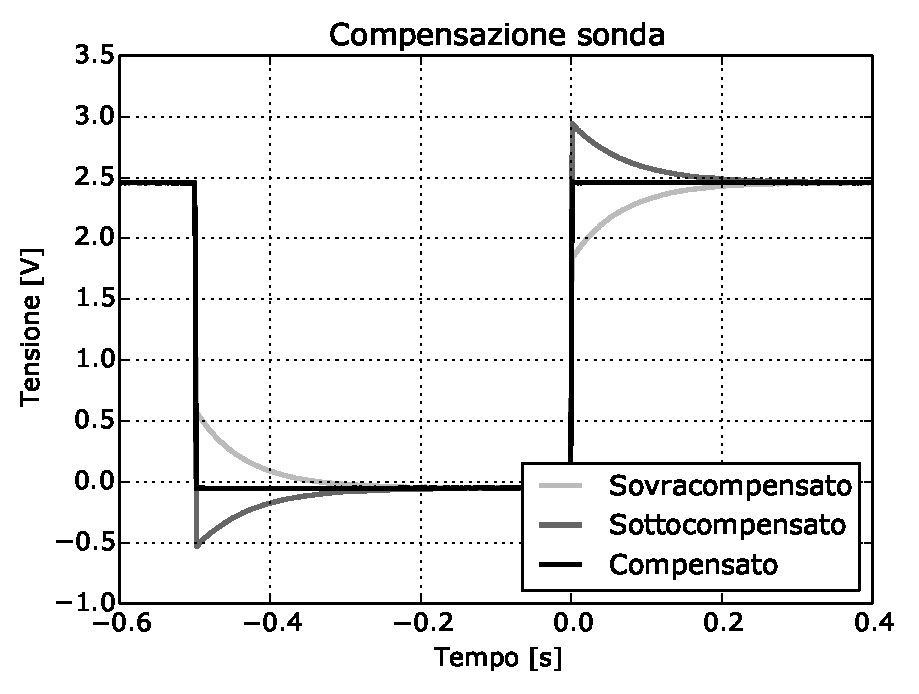
\includegraphics[width=\columnwidth]{figure/comp.pdf}
%    \caption{Input dell'oscilloscopio con una sonda compensabile. Cambiando capacità
%        si può ottenere una sottocompensazione, una sovracompensazione oppure compensare perfettamente
%        le capacità, ottenendo un'onda quadra.}
%    \label{fig:compensazione}
%\end{figure}

%\begin{wrapfloat}{figure}{O}{0pt}
%        \def\svgwidth{0.4\textwidth}
%        \subimport{figure/}{raddrizzatore.pdf_tex}
%        \caption{Raddrizzatore di precisione a semionda. Alimentato, inizialmente con una $V\ped{in}\,=\,\SI{1.02}{\volt}$ di frequenza $\nu\,=\,\SI{50}{\hertz}$.}
%        \label{fig:radd}
%\end{wrapfloat}

%\begin{SCfigure}[][p]
%        \centering
%        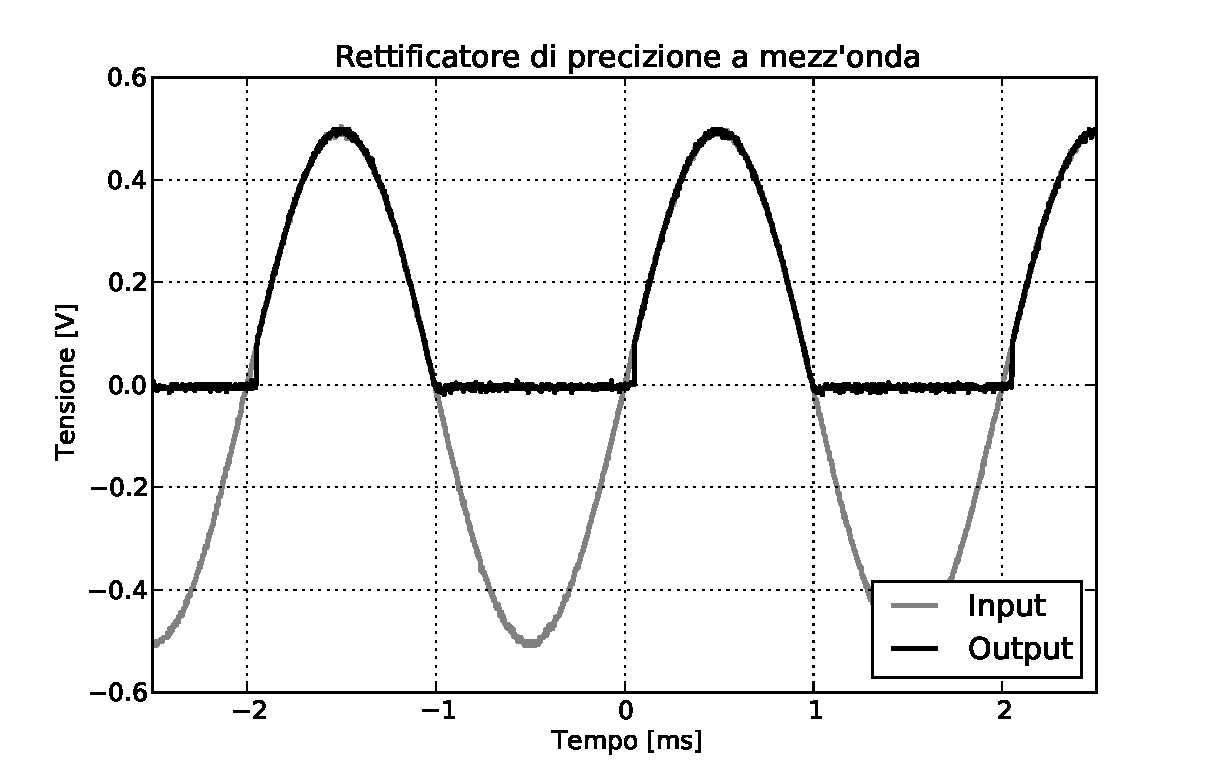
\includegraphics[width=0.7\textwidth]{figure/rett.pdf}
%        \caption{Questo grafico illustra l'andamento di $V\ped{out}$, linea nera, in funzione di $V\ped{in}$, linea grigia. Si nota chiaramente, come da previsioni, che la parte negativa del segnale in ingresso impediscse al diodo di condurre, pertanto la tensione di output risulta nulla. Inoltre, come si può osservare, il fronte di salita di $V\ped{out}$ presenta un leggero ritardo rispetto al segnale in ingresso $V\ped{in}$. Questo ritardo è stato stimato essere approssimativamente di circa $(152\pm10)\SI{}{\micro\second}$.}
%        \label{fig:radd_plot1}
%\end{SCfigure}
